%% This Beamer template is based on the one found here: https://github.com/sanhacheong/stanford-beamer-presentation, and edited to be used for Stanford ARM Lab

\documentclass[10pt]{beamer}
%\mode<presentation>{}

\usepackage{media9}
\usepackage{amssymb,amsmath,amsthm,enumerate}
\usepackage{mathtools}
\usepackage[utf8]{inputenc}
\usepackage{array}
\usepackage[parfill]{parskip}
\usepackage[utf8]{vietnam}
\usepackage{graphicx,animate}
\usepackage{caption}
\usepackage{subcaption}
\usepackage{bm}
\usepackage{amsfonts,amscd}
\usepackage[]{units}
\usepackage{listings}
\usepackage{multicol}
\usepackage{multirow}
\usepackage{tcolorbox}
\usepackage{physics}
\usepackage{movie15}
% Enable colored hyperlinks
\hypersetup{colorlinks=true}

% The following three lines are for crossmarks & checkmarks
\usepackage{pifont}% http://ctan.org/pkg/pifont
\newcommand{\cmark}{\ding{51}}%
\newcommand{\xmark}{\ding{55}}%

% Numbered captions of tables, pictures, etc.
\setbeamertemplate{caption}[numbered]
\usepackage{media9} 
%\usepackage[superscript,biblabel]{cite}
%\usepackage{algorithmic}
%\usepackage{algorithm2e}
%\usepackage{algpseudocode}
\usepackage[linesnumbered,ruled,vlined]{algorithm2e}
%\usepackage{algorithm}
%\usepackage{algorithmic}
\usepackage{caption}
%\usepackage{xcolor}
\usepackage{array}
%\renewcommand{\thealgocf}{}

\usepackage[natbib,backend=biber,style=ieee, sorting=ynt]{biblatex}
\bibliography{ref.bib}

\usepackage[acronym]{glossaries}

\usepackage{graphicx}
\graphicspath{{./figures}}
\usepackage{hyperref}

\theoremstyle{remark}
\newtheorem*{remark}{Remark}
\theoremstyle{definition}

%\newcommand{\empy}[1]{{\color{darkorange}\emph{#1}}}
%\newcommand{\empr}[1]{{\color{cardinalred}\emph{#1}}}
%\newcommand{\examplebox}[2]{
%\begin{tcolorbox}[colframe=darkcardinal,colback=boxgray,title=#1]
%#2
%\end{tcolorbox}}

%\usetheme{Stanford} 
%\def \i  {\item}
\def \ai {\item[] \quad \arrowbullet}
\newcommand \si[1]{\item[] \quad \bulletcolor{#1}}
\def \wi {\item[] \quad $\ \phantom{\Rightarrow}\ $}
\def \bi {\begin{itemize}\item}
\def \ei {\end{itemize}}
\def \be {\begin{equation*}}
\def \ee {\end{equation*}}
\def \bie {$\displaystyle{}
\def \eie {{\ }$}}
\def \bsie {\small$\displaystyle{}
\def \esie {{\ }$}\normalsize\selectfont}
\def \bse {\small\begin{equation*}}
\def \ese {\end{equation*}\normalsize}
\def \bfe {\footnotesize\begin{equation*}}
\def \efe {\end{equation*}\normalsize}
\renewcommand \le[1] {\\ \medskip \lefteqn{\hspace{1cm}#1} \medskip}
\def \bex {\begin{example}}
\def \eex {\end{example}}
\def \bfig {\begin{figure}}
\def \efig {\end{figure}}
\def \btheo {\begin{theorem}}
\def \etheo {\end{theorem}}
\def \bc {\begin{columns}}
\def \ec {\end{columns}}
\def \btab {\begin{tabbing}}
\def \etab {\end{tabbing}\svneg\svneg}
\newcommand \col[1]{\column{#1\linewidth}}
\def\vneg  {\vspace{-5mm}}
\def\lvneg {\vspace{-10mm}}
\def\svneg {\vspace{-2mm}}
\def\tvneg {\vspace{-1mm}}
\def\vpos  {\vspace{5mm}}
\def\lvpos {\vspace{10mm}}
\def\svpos {\vspace{2mm}}
\def\tvpos {\vspace{1mm}}
\def\hneg  {\hspace{-5mm}}
\def\lhneg {\hspace{-10mm}}
\def\shneg {\hspace{-2mm}}
\def\thneg {\hspace{-1mm}}
\def\hpos  {\hspace{5mm}}
\def\lhpos {\hspace{10mm}}
\def\shpos {\hspace{2mm}}

\usetheme{Copenhagen}
\usecolortheme{seahorse}
\logo{
\includegraphics[height=0.5in]{logos/HUS-name.jpg}}

\makeatletter
\let\@@magyar@captionfix\relax
\makeatother

\title[Trực quan hóa dữ liệu]{Trực quan hóa văn bản và tài liệu}

\AtBeginSection[]
{
    \begin{frame}
        \frametitle{Nội dung}
        \tableofcontents[currentsection, subsectionstyle=show/show/hide]
    \end{frame}
}

\setbeamertemplate{page number in head/foot}[totalframenumber]
\setbeamertemplate{frametitle continuation}{}

\begin{document}
\nocite{*}

\author[Nguyễn Chí Thanh - 21007925]{
	\begin{tabular}{c} 
	\Large
	Nguyễn Chí Thanh \\
    \footnotesize \href{mailto:nguyenchithanh\_sdh21@hus.edu.vn}{nguyenchithanh\_sdh21@hus.edu.vn}
\end{tabular}
\vspace{-4ex}}

\institute{
	\vskip 5pt
	\begin{figure}
		\centering
		\begin{subfigure}[t]{0.5\textwidth}
			\centering
			
\includegraphics[height=0.75in]{logos/HUS-logo.jpg}
		\end{subfigure}%
		~ 
		\begin{subfigure}[t]{0.5\textwidth}
			\centering
			
\includegraphics[height=0.75in]{logos/MIM-logo.png}
		\end{subfigure}
	\end{figure}
	\vskip 5pt	
	Đại học Quốc Gia Hà Nội \\
	Trường đại học Khoa học tự nhiên\\
	Khoa Toán - Cơ - Tin học
	\vskip 3pt
}

%\begin{noheadline}
\begin{frame} \maketitle \end{frame}
%\end{noheadline}
    
\setbeamertemplate{itemize items}[default]
\setbeamertemplate{itemize subitem}[circle]

\begin{frame}{Nội dung}
    \tableofcontents[hidesubsections]
\end{frame}

\section{Các cấp biểu diễn văn bản}

\begin{frame}{Các cấp biểu diễn văn bản}
	\begin{figure}[h!]
        \centering
        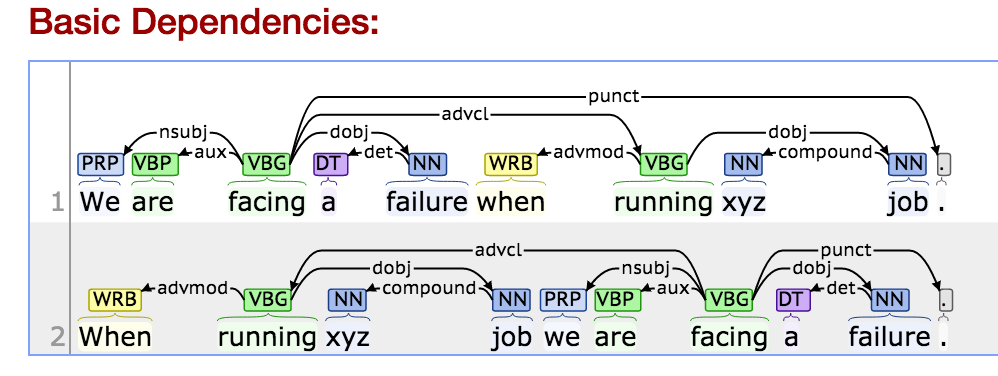
\includegraphics[width=0.8\textwidth]{QlGQ3.png}
        \caption{Minh họa các cấp độ biểu diễn văn bản}
        \label{fig:Dependency-Parsing}
    \end{figure}
\end{frame}

\subsection{Cấp độ từ vựng}

\begin{frame}{Cấp độ từ vựng}
	\begin{itemize}
		\item Cấp độ từ vựng liên qua đến việc biến đổi một chuỗi các ký tự sang một dãy các thực thể nguyên tử được gọi là \textit{tokens}.
		\item Bộ phân tích từ vựng xử lý dãy các ký tự với một bộ quy tắc nhất định thành một dãy các tokens mới có thể được sử dụng cho những phân tích sâu hơn.
		\item Tokens có thể bao gồm các ký tự, các ký tự n-grams, các từ, các gốc từ, các từ vựng, các cụm từ.
	\end{itemize}
    
\end{frame}

\subsection{Cấp độ cú pháp}

\begin{frame}{Cấp độ cú pháp}
	\begin{itemize}
		\item Cấp độ cú pháp liên quan đến việc xác định và gắn thẻ (chú thích) cho từng chức năng của tokens
		\item Quá trình trích xuất các gán nhãn này được gọi là \textit{nhận diện thực thể được đặt tên} (NER).
	\end{itemize}
\end{frame}

\subsection{Cấp độ ngữ nghĩa}

\begin{frame}{Cấp độ ngữ nghĩa}
	\begin{itemize}
		\item Cấp độ ngữ nghĩa bao gồm việc trích xuất xuất các ý nghĩa và quan hệ giữa các phần tri thức thu được từ các cấu trúc được xác định ở cấp độ cú pháp.
	\end{itemize}
\end{frame}

\section{Mô hình không gian vector}

\begin{frame}{Mô hình không gian vector}
	\begin{itemize}
		\item  Tính toán vectors các thuật ngữ hoặc các từ là một bước thiết yếu cho nhiều kỹ thuật trực quan hóa và phân tích tài liệu và văn bản.
		\item Trong \textit{mô hình không gian vector} \cite{356}, một vector của một thuật ngữ hoặc một từ cho một đối tượng quan tâm (đoạn văn, tài liệu hoặc một tập các tài liệu) là một vector mà trong đó mỗi chiều biểu diễn trọng số của một từ đã cho trong tài liệu đó.
		\item Thông thường, để loại bỏ nhiễu hoặc các từ dừng (stop words) (ví dụ "the", "a") được loại bỏ (lọc) và các từ có chung gốc được ghép vào làm một (ghép từ gốc).
	\end{itemize}
\end{frame}


\begin{frame}{Mô hình không gian vector}
	\begin{algorithm}[H]
        \DontPrintSemicolon
        $terms \gets \emptyset$\;
        \ForEach{$token$ $t$ \textbf{in} $tokenStream$}{
            \If{$t$ không phải là một từ dừng}{
                \If{$t$ \textbf{not in} $terms$} {
                    $terms \lbrack t \rbrack \gets 1$\;
                } 
                \Else {
                    $terms \lbrack t \rbrack \gets terms \lbrack t \rbrack + 1$\;
                }
            }
        }
        \Return{$terms$}\;
        \caption{COUNT-TERMS(tokenStream)}
        \label{alg:COUNT-TERMS}
    \end{algorithm}
\end{frame}

\begin{frame}{Mô hình không gian vector}
	\begin{table}[h!]
		\resizebox{10cm}{!}{%
        \begin{tabular} {|c| c| c| c| c| c| c| c| c| c|}
            \hline
            genetically & said & safety & engineered & study & test & great & deal & controversy & foods \\
            \hline
            3 & 3 & 2 & 2 & 2 & 2 & 1 & 1 & 1 & 1 \\
            \hline
        \end{tabular}
		}
    \end{table}
\end{frame}

\subsection{Tính toán các trọng số}

\begin{frame}{Tính toán các trọng số}
	\begin{itemize}
		\item Mô hình không gian vector yêu cầu một sơ đồ trọng số để gán trọng số cho các thuật ngữ ở trong một tài liệu.
		\item Có nhiều phương pháp để làm việc này, phương pháp nổi tiếng nhất trong số đó là tần số thuật ngữ - tần số tài liệu nghịch đảo (tf-idf) \cite{355}.
		\item  $Tf(w)$ là tần suất của thuật ngữ hay số lần mà từ $w$ xuất hiện trong tài liệu, và $Df(w)$ là tần suất của tài liệu (số tài liệu có chứa từ đó).
		Gọi $N$ là số tài liệu. Ta tính $TfIdf(w)$ theo công thức:
		\begin{equation}
			TfIdf(w) = Tf(w) \times \log \Big( \dfrac{N}{Df(w)} \Big)
		\end{equation}
	\end{itemize}
\end{frame}

\begin{frame}{Tính toán các trọng số}
	Mã giả ở thuật toán \ref{alg:COMPUTE-TFIDF} tính toán các vector tf-idf cho từng tài liệu.
	\resizebox{3.5cm}{!}{%
	\begin{algorithm}[H]
        \DontPrintSemicolon
        $termFrequencies \gets \emptyset$\; \tcp{Tra cứu bảng đếm số lần thuật ngữ/từ xuất hiện cho tên tài liệu}
        $documentFrequencies \gets  \emptyset$\; \tcp*{Đếm số tài liệu mà trong đó một thuật ngữ/từ nhất định xuất hiện}
        $uniqueTerms \gets \emptyset$\; \tcp*{Danh sách các thuật ngữ/từ riêng biệt}
        \ForEach{$document$ $d$ \textbf{in} $documents$}{
            $docName \gets NAME(d)$\; \tcp{Trích xuất tên của tài liệu}
            $tokenStream \gets TOKENIZE(d)$\; \tcp{Tạo luồng token của tài liệu}
            $terms \gets COUNT-TERMS(tokenStream)$\; \tcp{Đếm tần suất của các thuật ngữ/từ}
            $termFrequencies \lbrack docName \rbrack \gets terms$\; \tcp{Lưu trữ tần suất các thuật ngữ/từ tương ứng với từng tài liệu}
            \ForEach{$term$ $t$ \textbf{in} $KEYS(terms$)}{
                \If{$t$ \textbf{not in} $documentFrequencies$} {
                    $documentFrequencies \lbrack t \rbrack \gets 1$\;
                } 
                \Else {
                    $documentFrequencies \lbrack t \rbrack \gets documentFrequencies \lbrack t \rbrack + 1$\;
                }
                $uniqueTerms \gets uniqueTerms \cup t$\;
            }
        }
        $tfIdfVectorTable \gets \emptyset$\; \tcp{Tra cứu vector tf-idf cho tên tài liệu}
        $n \gets LENGTH(documents)$\;
        \ForEach{$document$ $name$ $docName$ \textbf{in} $KEYS(termFrequencies)$}{
            $tfIdfVector \gets $ \text{zeroes array of length} $LENGTH(uniqueTerms)$\;
            $terms \gets termFrequencies \lbrack docName \rbrack$\;
            \ForEach{$term$ $t$ \textbf{in} $KEYS(terms)$}{
                $tf \gets terms \lbrack t \rbrack$\;
                $df \gets documentFrequencies \lbrack t \rbrack$\;
                $tfIdf \gets tf \times \log \Big( \dfrac{n}{df} \Big)$\;
                $tfIdfVector \lbrack \text{chỉ số của } t \text{ trong } uniqueTerms \rbrack \gets tfIdf$\;
            }
            $tfIdfVectorTable \lbrack docName \rbrack \gets tfIdfVector$\;
        }
        \Return{$tfIdfVectorTable$}\;
        \caption{COMPUTE-TFIDF(documents)}
        \label{alg:COMPUTE-TFIDF}
    \end{algorithm}
	}
\end{frame}


\begin{frame}
	\begin{figure}[h!]
        \centering
        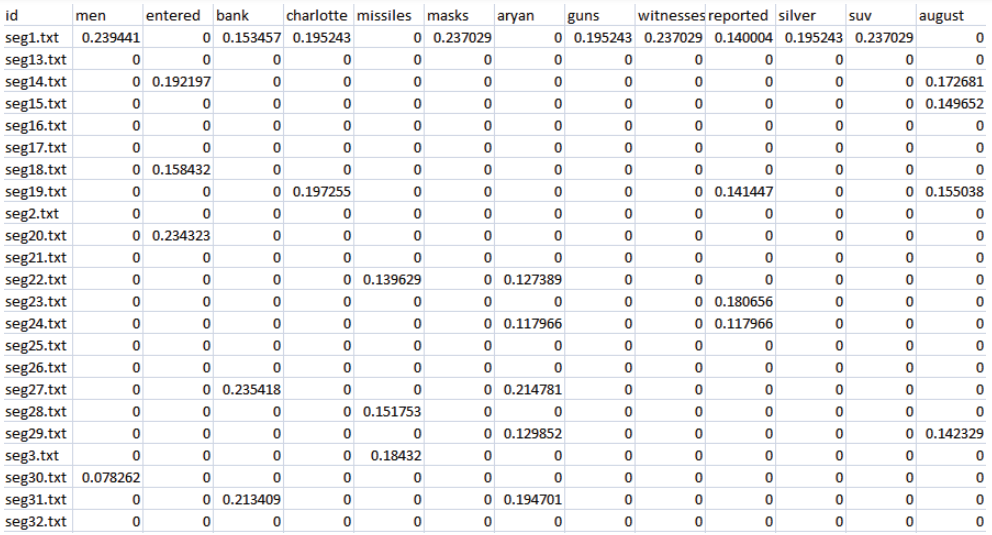
\includegraphics[width=0.8\textwidth]{1.png}
        \caption{Minh họa của các vector của các thuật ngữ trong nhiều tài liệu, bao gồm giá trị tf-idf.}
        \label{fig:1}
    \end{figure}
\end{frame}

\subsection{Định luật Zipf}

\begin{frame}{Định luật Zipf}
	\begin{itemize}
		\item Phân phối chuẩn và phân phối đều là các phân phối ta quen thuộc nhất.
		\item Phân phối hàm mũ ngày nay rất phổ biến với kích thước dữ liệu lớn, phản ánh hiện tượng mở rộng dữ liệu.
		\item Nhà kinh tế học Vilfredo Pareto tuyên bố rằng doanh thu của một công ty tỷ lệ nghịch với thứ hạng của công ty này, chính là tuân theo phân phối mũ kinh điển,
		dẫn đến quy tắc 80 - 20, trong đó 20\% dân số nắm giữ 80\% tài sản
	\end{itemize}
	
\end{frame}

\begin{frame}{Định luật Zipf}
	\begin{figure}[h!]
        \centering
        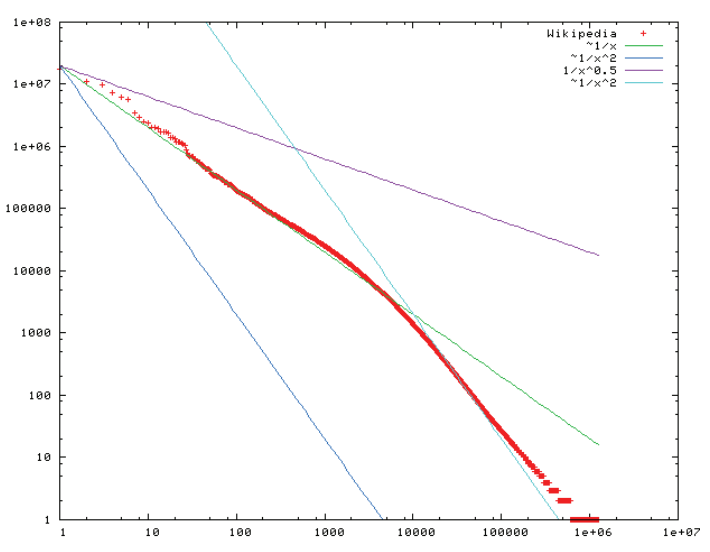
\includegraphics[width=0.6\textwidth]{2.png}
        \caption{Phân phối của các thuật ngữ trong Wikipedia, một ví dụ về luật Zipf.
        Phân phối của các thuật ngữ nằm trên trục y, và thứ hạng tần suất nằm trên trục x.}
        \label{fig:2}
    \end{figure}

\end{frame}

\begin{frame}{Định luật Zipf}
	\begin{itemize}
		\item Phân phối của các từ trong corpora tuân theo phân phối mũ được gọi là phân phối Zipf.
		\item Định luật Zipf \cite{490} phát biểu rằng trong một tài liệu ngôn ngữ tự nhiên điển hình, tần suất của một từ tỷ lệ nghịch với thứ hạng của nó trong bảng tần suất.
		\item Vẽ đồ thị đường cong Zipf trên thang đo log - log ta thu được một đường thẳng có hệ số góc -1 (hình \ref{fig:2}).
		\item Ý nghĩa của định luật Zipf là một lượng nhỏ các từ miêu tả hầu hết các khái niệm chính trong các tài liệu nhỏ.
	\end{itemize}
\end{frame}

\subsection{Các nhiệm vụ sử dụng mô hình không gian vector}

\begin{frame}{Các nhiệm vụ sử dụng mô hình không gian vector}
	\begin{itemize}
		\item Mô hình không gian vector, khi đi cùng với một độ đo khoảng cách cho phép ta thực hiện nhiều tác vụ hữu ích.
		\item Ta có thể sử dụng tf-idf và mô hình không gian vector để nhận diện các tài liệu cần được quan tâm đặc biệt.
		\item Ví dụ, mô hình không gian vector, với việc sử dụng một số độ đo khoảng cách, sẽ cho phép ta trả lời câu hỏi tài liệu nào giống với một tài liệu cụ thể cho trước.
		\item Làm thế nào để giúp người dùng hiểu được ý nghĩa của toàn bộ corpus.
		\item Biến đổi các tà liệu này thành các vector, sau đó thực thi các thuật toán dựa trên các nhiệm vụ đang được quan tâm (đo độ tương tự, tìm kiếm, phân cụm) và thực hiện trực quan hóa.
	\end{itemize}
\end{frame}

\section{Trực quan hóa tài liệu đơn}

\subsection{Đám mây từ (Wordcloud)}

\begin{frame}{Đám mây từ (Wordcloud)}
	\begin{figure}[h!]
        \centering
        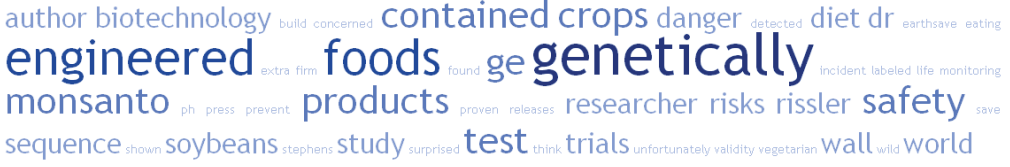
\includegraphics[width=0.95\textwidth]{4.png}
        \caption{Trực quan hóa đám mây thẻ được tạo bởi dịch vụ miễn phí tagCrowd.com \cite{396}.
        Cỡ chữ và độ tối tỷ lệ thuận với tuần suất xuất hiện của từ trong tài liệu}
        \label{fig:4}
    \end{figure}
\end{frame}

\begin{frame}{Đám mây từ (Wordcloud)}
	\begin{figure}[h!]
        \centering
        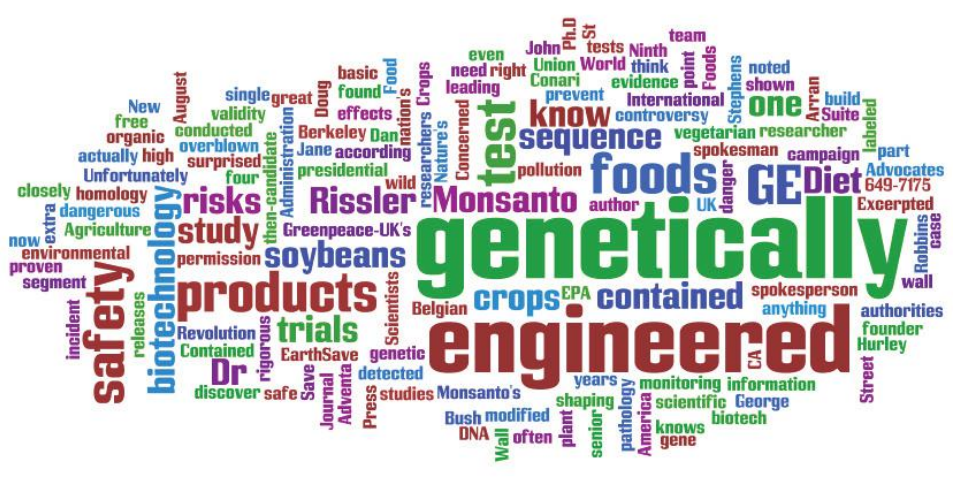
\includegraphics[width=0.8\textwidth]{5.png}
        \caption{Một Wordle được tạo bởi dịch vụ miễn phí wordle.net \cite{118}.
        Kích thước của các từ tương ứng với tần suất của từ trong tài liệu}
        \label{fig:5}
    \end{figure}
\end{frame}


\begin{frame}{Đám mây từ (Wordcloud)}
	\begin{itemize}
		\item Đám mây từ (hình \ref{fig:4}), còn được gọi là đám mây văn bản hoặc đám mây thẻ, là bố của các các token mà được tô màu và định cỡ hiển thị theo tần suất xuất hiện của chúng trong một tài liệu.
		\item Có một vài biến thể, ví dụ là Wordle
	\end{itemize}
\end{frame}

\subsection{WordTree}

\begin{frame}{WordTree}
	\begin{itemize}
		\item Trực quan hóa WordTree \cite{450} là một biểu diễn trực quan của cả tần số thuật ngữ cũng như ngữ cảnh của thuật ngữ (hình \ref{fig:6}).
		\item Kích thước được sử dụng để đại diện cho thuật ngữ hoặc tần suất của cụm từ.
		\item Gốc của cây là một từ hoặc cụm từ do người dùng chỉ định và các nhánh biểu diễn các ngữ cảnh khác nhau mà từ hoặc cụm từ được sử dụng trong tài liệu.
	\end{itemize}
\end{frame}

\begin{frame}{WordTree}
	\begin{figure}[h!]
        \centering
        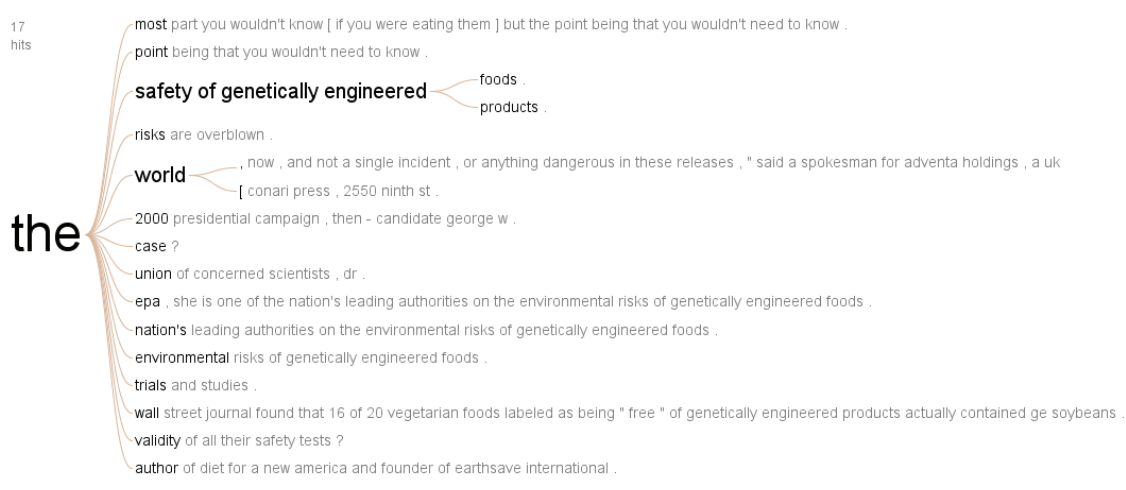
\includegraphics[width=0.8\textwidth]{6.png}
        \caption{Hình ảnh WordTree được tạo bởi dịch vụ miễn phí ManyEyes \cite{196}.
        Các nhánh của cây đại diện cho các ngữ cảnh khác nhau theo sau một từ gốc hoặc cụm từ gốc trong tài liệu}
        \label{fig:6}
    \end{figure}
\end{frame}

\subsection{TextArc}

\begin{frame}{TextArc}
	\begin{itemize}
		\item Ta có thể mở rộng biểu diễn của phân phối từ bằng cách hiển thị kết nối.
		\item Có nhiều cách để tính toán kết nối giữa các từ.
		\item TextArc \cite{312} là một biểu diễn trực quan về các thuật ngữ liên quan đến dòng văn bản mà nó xuất hiện (hình \ref{fig:7}).
		\item Mỗi từ trong văn bản được vẽ theo thứ tự xung quan một elip dưới dạng các dòng nhỏ với độ lệch nhẹ ở đầu.
		\item Cũng như trong đám mấy văn bản, các từ với tần suất cao hơn được vẽ lớn hơn và sáng hơn.
	\end{itemize}
\end{frame}

\begin{frame}{TextArc}
	\begin{figure}[h!]
        \centering
        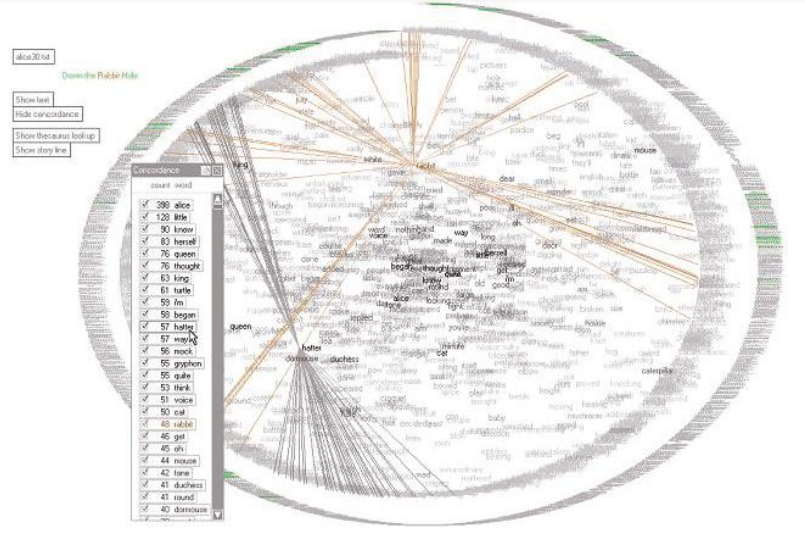
\includegraphics[width=0.7\textwidth]{7.png}
        \caption{Một hình ảnh TextArc được tạo ra sử dụng truyện "Alice in Wonderland".
        Các từ xuất hiện trong toàn bộ các phần trong tài liệu được đặt ở giữa TextArc, trong khi các từ chỉ xuất hiện trong vài phần cụ thể được đặt gần viền hơn.}
        \label{fig:7}
    \end{figure}
\end{frame}

\subsection{Sơ đồ vòng cung (Arc Diagrams)}

\begin{frame}{Sơ đồ vòng cung (Arc Diagrams)}
	\begin{itemize}
		\item Sơ đồ vòng cung là trực quan hóa tập trung vào việc hiển thị sự lặp lại trong văn bản.
		\item Các dãy con lặp đi lặp lại được xác định và được nối với nhau bằng các cung nửa hình tròn.
		\item Độ dày của các cung biểu diễn độ dài của các dãy con và độ cao của các cung biểu diễn khoảng cách giữa các dãy con.
		\item Hình \ref{fig:8} hiển thị "Bach’s Minuet in G Major", trực quan hóa mô hình cổ điển của điệu nhảy Minuet.
	\end{itemize}
\end{frame}

\begin{frame}{Sơ đồ vòng cung (Arc Diagrams)}
	\begin{figure}[h!]
        \centering
        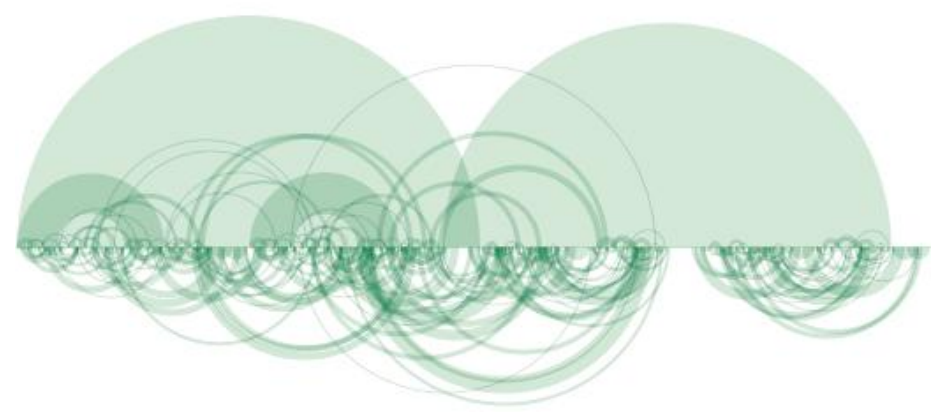
\includegraphics[width=0.9\textwidth]{8.png}
        \caption{Một hình ảnh sơ đồ vòng cung của "Bach’s Minuet in G Major".
        Các dãy lặp lại được kết nối bằng một đường cong nửa hình tròn. \cite{451}}
        \label{fig:8}
    \end{figure}
\end{frame}

\subsection{Dấu ấn văn học (Literature Fingerprinting)}

\begin{frame}{Dấu ấn văn học (Literature Fingerprinting)}
	\begin{itemize}
		\item Dấu ấn văn học là một phương pháp trực quan hóa các đặc trưng được sử dụng để thể hiện các đặc tính của văn bản \cite{222}.
		\item Thay vì chỉ tính toán một giá trị đặc trưng hoặc một vector cho toàn bộ văn bản (đây là điều hay thường được thực hiện), ta tính toán một dãy các giá trị đặc trưng từng văn bản và hiển thị chúng cho người dùng dưới dạng dấu ấn đặc trưng của tài liệu.
		\item Thông tin cấu trúc của tài liệu được dùng để trực quan hóa tài liệu trên nhiều cấp độ khác nhau của độ phân giải.
		\item Dấu ấn văn học được áp dụng cho bài toán xác nhận quyền tác giả để thể hiện khả năng phân biệt của các độ đo tiêu chuẩn được giả định để nắm bắt được phong cách sáng tác của một tác giả (hình \ref{fig:9}).
	\end{itemize}
\end{frame}

\begin{frame}{Dấu ấn văn học (Literature Fingerprinting)}
	\begin{figure}[h!]
        \centering
        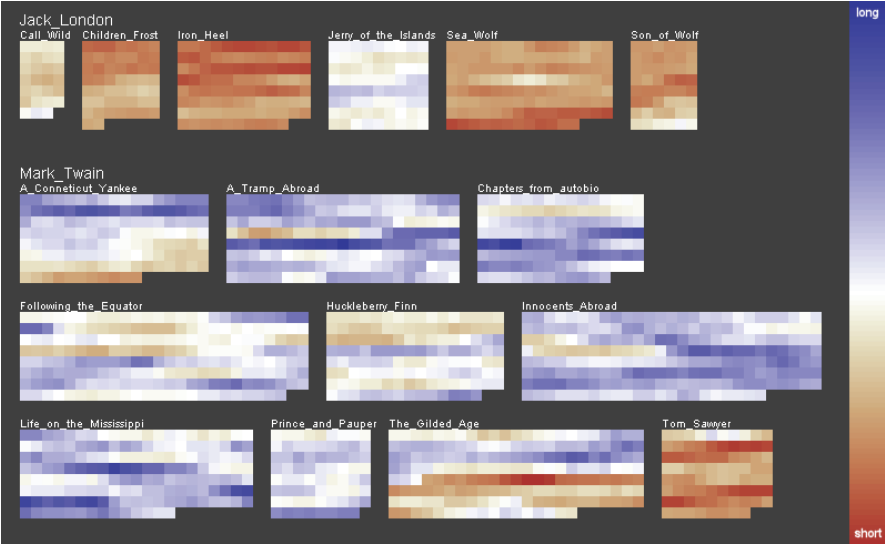
\includegraphics[width=0.6\textwidth]{9.png}
        \caption{Kỹ thuật lấy dấu ấn văn học. Dấu ấn văn học được sử dụng để phân tích nhiều độ đo văn bản để phân biệt tác giả của tài liệu.
        Từng điểm ảnh biểu diễn một khối văn bản, các điểm ảnh được ghép lại thành các cuốn sách.
        Màu các điểm ảnh được ảnh xạ từ các giá trị đặc trưng, trong trường hợp này là độ dài trung bình của câu.
        Nếu một độ đo có khả năng phân biệt giữa hai tác giả, các sách ở hàng đầu tiên được viết bởi Jack London và các sách còn lại được viết bởi Mark Twain. \cite{222}}
        \label{fig:9}
    \end{figure}
\end{frame}


\section{Trực quan hóa tập tài liệu}

\begin{frame}{Trực quan hóa tập tài liệu}
	\begin{itemize}
		\item Trong hầu hết các trường hợp trực quan hóa tập tài liệu, mục tiêu đặt ra là đặt các tài liệu tương tự nhau ở gần nhau và các tài liệu khác nhau cách xa nhau.
		\item Đây là bài toán thường có độ phức tạp $O(n^2)$.
		\item Ta tính toán sự giống nhau giữa tất cả từng cặp tài liệu và xác định bố cục.
		\item Cách tiếp cẩn phổ biến là đồ thị, phân cụm (k-means, phân cấp, tối đa hóa kỳ vọng (EM), vector hỗ trợ) và bản đồ tự tổ chức.
	\end{itemize}
\end{frame}

\subsection{Bản đồ tự tồ chức}

\begin{frame}{Bản đồ tự tồ chức}
	\begin{itemize}
		\item Bản đồ tự tổ chức (SOM) \cite{248} là một thuật toán học không giám sát bằng cách sử dụng một tập các nút thường là 2 chiều, vị trí mà tài liệu sẽ được đặt.
		\item Từng nút có một vector tương ứng với cùng số chiều với vector đầu vào (các vector tài liệu) được sử dụng để huấn luyện bản đồ.
		\item Ta khởi tạo các nút của SOM, thường có các trọng số ngẫu nhiên.
		\item Ta chọn một vector ngẫu nhiên từ các vector đầu vào và tính toán khoảng cách của nó đến từng mỗi nút khác.
		\item Ta điều chỉnh trọng số của các nút gần nhất (trong một bán kính cụ thể), làm cho mỗi nút gần hơn tới vector đầu vào,
		với trọng số đầu vào cao hơn tương ứng với nút được chọn gần nhất.
		\item Khi ta lặp qua các vector đầu vào, bán kính sẽ nhỏ hơn.
	\end{itemize}
\end{frame}

\begin{frame}{Bản đồ tự tồ chức}
	\begin{figure}[h!]
        \centering
        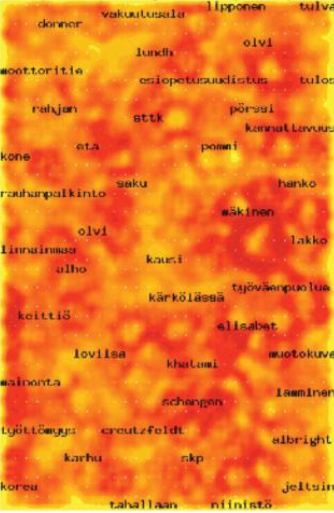
\includegraphics[width=0.3\textwidth]{10.png}
        \caption{Bố cục bản đồ tự tổ chức của mục bản tin Phần Lan.
        Các nhãn hiển thị các khu vực chủ đề và màu sắc biểu thị số lượng các tài liệu tương ứng với chủ đề, với các vùng càng sáng chứa nhiều tài liệu hơn \cite{454}.}
        \label{fig:10}
    \end{figure}
\end{frame}

\subsection{Hình nền chủ đề}

\begin{frame}{Hình nền chủ đề}
	\begin{itemize}
		\item Hình nền chủ đề là bản tóm tắt của corpora sử dụng phong cảnh 3 chiều trừu tượng, trong đó chiều cao và màu sắc được sử dụng để biểu diễn mật độ của các tài liệu tương tự giống nhau.
		\item Một ví dụ được minh họa trong hình \ref{fig:11} từ Pacific Northwest National Labs \cite{407} đại diện cho các bài báo được trực quan hóa dưới dạng hình nền chủ đề.
		\item Các ngọn núi cao hơn biểu thị tần suất chủ đề cao hơn trong kho tài liệu (chiều cao tỷ lệ thuận với số lượng tài liệu liên quan đến chủ đề).
	\end{itemize}
\end{frame}

\begin{frame}{Hình nền chủ đề}
	\begin{figure}[h!]
        \centering
        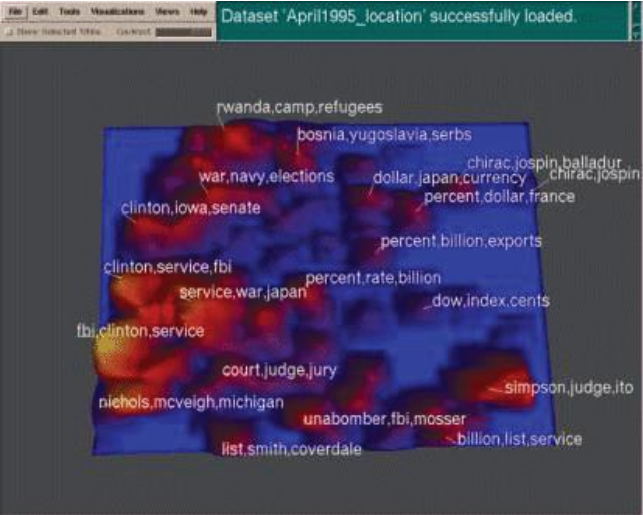
\includegraphics[width=0.5\textwidth]{11.png}
        \caption{Một hình nền chủ đề từ PNNL sử dụng chiều cao để biểu diễn tần suất xuất hiện của các chủ đề trong các bài báo. (Hình ảnh được in từ \cite{407} với sự cấp phép của  Springer Science and Business Media).}
        \label{fig:11}
    \end{figure}
\end{frame}

\subsection{Thẻ tài liệu}

\begin{frame}{Thẻ tài liệu}
	\begin{itemize}
		\item Thẻ tài liệu là một cách trực quan hóa thu gọn (hình \ref{fig:12}) biểu diễn ngữ nghĩa chính của tài liệu dưới dạng hỗn hợp hình ảnh và các thuật ngữ chính quan trọng, tương tự như thẻ trong trò chơi át chủ bài \cite{400}.
		Các thuật ngữ chính được trích xuất bằng cách sử dụng một cách tiếp cận khai phá văn bản nâng cao dựa trên trích xuất tự động của cấu trúc tài liệu.
		\item Các thuật ngữ chính được trích xuất bằng cách sử dụng một cách tiếp cận khai phá văn bản nâng cao dựa trên trích xuất tự động của cấu trúc tài liệu.
		\item Phân phối màu của ảnh được dùng để phân loại hình ảnh vào các lớp (lớp 1: ảnh chụp/ảnh kết xuất, lớp 2: sơ đồ/bản phác thảo/đồ thị, lớp 3: bảng) và hiển thị ít nhất một đại diện từ mỗi lớp không rỗng.
	\end{itemize}
\end{frame}

\begin{frame}{Thẻ tài liệu}
	\begin{figure}[h!]
        \centering
        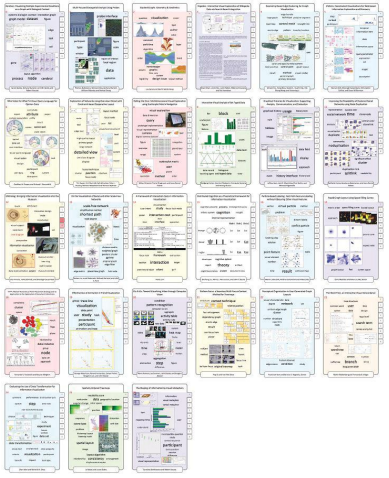
\includegraphics[width=0.35\textwidth]{12.png}
        \caption{Kho tài liệu của hội nghị IEEE InfoVis 2008 được biểu diễn bằng một ma trận các thẻ tài liệu.
        Tuần suất của các thuật ngữ trên từng trang được hiển thị ở bên tay phải của thẻ lại liệu (màu càng đỏ thể hiện tần suất càng cao, ta có thể thấy ở tài liệu thứ nhất ở hàng thứ 3) \cite{400}.}
        \label{fig:12}
    \end{figure}
\end{frame}

\section{Các kỹ thuật trực quan hóa văn bản mở rộng}

\subsection{Trực quan hóa phần mềm}

\begin{frame}{Trực quan hóa phần mềm}
	\begin{itemize}
		\item Eick và các cộng sự đã phát triển một công cụ trực quan hóa có tên là SeeSoft \cite{108} giúp trực quan hóa số liệu thống kê cho từng dòng code (tuổi và số thay đổi, lập trình viên, ngày tháng).
		\item Hình \ref{fig:13}, từng cột biểu diễn một file mã nguồn với chiều cao biểu thị kích thước của file.
		\item Nếu như file dài hơn màn hình, nó sẽ tiếp tục được biểu diễn ở cột tiếp theo.
		\item Trong biểu diễn của SeeSoft, từng hàng biểu diễn một dòng code.
	\end{itemize}
\end{frame}

\begin{frame}{Trực quan hóa phần mềm}
	\begin{itemize}
		\item Vì số lượng dòng quá lớn cho một hàng, nên mỗi dòng được biểu diễn bởi một điểm ảnh trong hàng ngang.
		\item Màu sắc được sử dụng để biểu thị số lần được gọi.
		\item Dòng càng màu đỏ thì dòng này càng được gọi nhiều, được gọi là điểm nóng (key hotspot).
		\item Một dòng màu xanh thể hiện ít được gọi hơn.
	\end{itemize}
\end{frame}

\begin{frame}{Trực quan hóa phần mềm}
	\begin{figure}[h!]
        \centering
        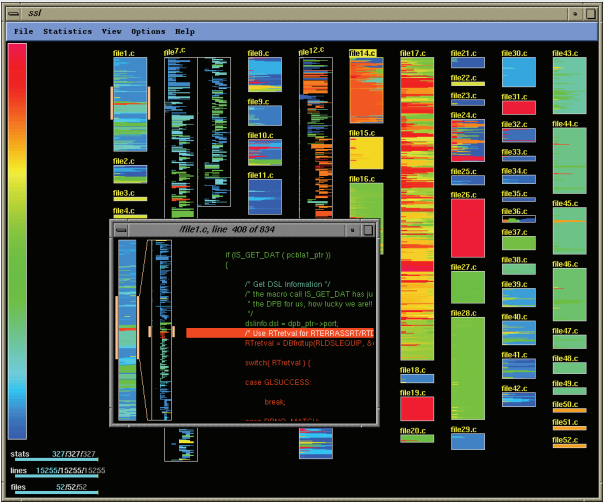
\includegraphics[width=0.5\textwidth]{13.png}
        \caption{Trực quan hóa sử dụng phần mềm SeeSoft. Các hình chữ nhật biểu diễn các file mã nguồn.
        Kích thước của các hình chữ nhật trong từng cột tương ứng với độ dài của file mã nguồn, và màu sắc của từng dòng biểu diễn các tham số liên quan đến việc sửa đổi \cite{108}.}
        \label{fig:13}
    \end{figure}
\end{frame}

\subsection{Trực quan hóa kết quả truy vấn}

\begin{frame}{Trực quan hóa kết quả truy vấn}
	\begin{itemize}
		\item Marti Hearst đã phát triển một công cụ trực quan hóa kết quả truy vấn đơn giản về cơ bản tương tự như của \cite{232} được gọi là TileBars \cite{178}.
		hiển thị một số thống kê liên quan đến thuật ngữ, bao gồm tần suất và phân phối của thuật ngữ, độ dài của tài liệu, xếp hạng dựa trên thuật ngữ và sức mạnh của xếp hạng.
		\item  Mỗi tài liệu của tập kết quả được biểu diễn bằng một hình chữ nhật, trong đó chiều rộng biểu thị chiều dài tương dối của tài liệu và các ô vuông xếp chồng tương ứng với các đoạn văn bản (hình \ref{fig:14}).
		\item Mỗi hàng của ngắn xếp đại diện cho tập các thuật ngữ truy vấn và mức độ tối của hình vuông thể hiện tần suất của các thuật ngữ trong số các thuật ngữ tương ứng.
		\item Tiêu đề và những từ mở đầu từ tài liệu xuất hiện bên cạnh TileBar.
	\end{itemize}
\end{frame}

\begin{frame}{Trực quan hóa kết quả truy vấn}
	\begin{itemize}
		\item  Mỗi hình chữ nhật lớn biểu diễn một văn bản, mỗi hình vuông trong tài liệu biểu diễn một đoạn văn bản.
		\item Ô càng tối thì tập hợp thuật ngữ truy vấn càng có tần suất lớn.
		\item Điều này tạo ra một biểu diễn thu gọn và cung cấp các phản hồi về cấu trúc tài liệu phản ánh độ dài tương đối của tài liệu,
		tần suất của thuật ngữ truy vấn và phân phối của các thuật ngữ truy vấn.
	\end{itemize}
\end{frame}


\begin{frame}{Trực quan hóa kết quả truy vấn}
	\begin{figure}[h!]
        \centering
        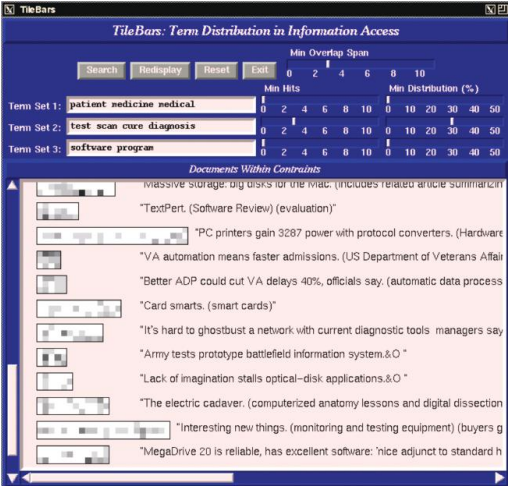
\includegraphics[width=0.5\textwidth]{14.png}
        \caption{Trực quan hóa kết quả truy vấn TileBars.
        Mỗi hình chữ nhật lớn biểu thị một tài liệu, mỗi hình vuông bên trong tài liệu biển diễn một đoạn văn bản.
        Ô càng tối thì tập hợp thuật ngữ truy vấn có tần suất càng lớn \cite{178}.}
        \label{fig:14}
    \end{figure}
\end{frame}

\subsection{Trực quan hóa tập tài liệu theo thời gian}

\begin{frame}{Trực quan hóa tập tài liệu theo thời gian}
	\begin{itemize}
		\item ThemeRiver \cite{173} còn được gọi là biểu đồ luồng, là một kỹ thuật trực quan hóa các thay đổi chủ đề theo thời gian trong tập tài liệu (hình \ref{fig:15}).
		\item Hình ảnh trực quan này giả định rằng dữ liệu đầu vào thay đổi theo thời gian.
		\item Các chủ đề được thể hiện trực quan dưới dạng các dải màu nằm ngang có độ dày theo chiều dọc ở một vị trí theo chiều ngang nhất định biểu diễn tần suất của tại một thời điểm cụ thể.
	\end{itemize}
\end{frame}

\begin{figure}[h!]
	\centering
	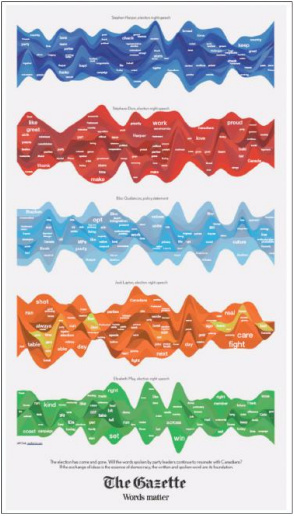
\includegraphics[width=0.35\textwidth]{15.png}
	\caption{Biểu đồ luồng (ThemeRiver) miêu tả các bài phát biểu trong đêm bầu cử của một số ứng viên khác nhau cho cuộc bầu cử ở Canada \cite{173}.}
	\label{fig:15}
\end{figure}

\begin{frame}{Trực quan hóa tập tài liệu theo thời gian}
	\begin{itemize}
		\item Jigsaw là một công cụ để trực quan hóa và khám phá kho văn bản \cite{155}.
		\item Chế độ xem lịch định vị các đối tượng tài liệu dựa trên các thực thể ngày tháng được xác định trong văn bản.
		\item Khi người dùng ấn vào một tài liệu, các thực thể sẽ xuất hiện trong tài liệu đó sẽ được hiển thị (hình \ref{fig:16}.)
	\end{itemize}
\end{frame}

\begin{frame}{Trực quan hóa tập tài liệu theo thời gian}
	\begin{figure}[h!]
        \centering
        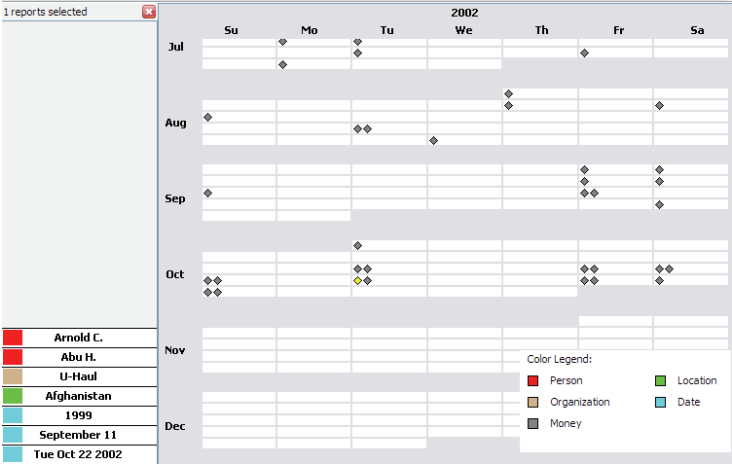
\includegraphics[width=0.65\textwidth]{16.png}
        \caption{Các bài báo được trình bày dưới dạng xem lịch Jigsaw, dựa trên các thực thể ngày được trích xuất \cite{155}.}
        \label{fig:16}
    \end{figure}
\end{frame}

\begin{frame}{Trực quan hóa tập tài liệu theo thời gian}
	\begin{itemize}
		\item Wanner và các đồng sự phát triển một công cụ phân tích trực quan để tiến hành phân tihcs cảm xúc bán tự động từ các nguồn tin tức lớn.
		\item Mặc dù công cụ này tự động thu thập và phân tích từ nguồn RSS liên quan đến các từ có quan điểm tích cực và tiêu cực, nhưng việc phân tích tin tức đòi hỏi khắt khe hơn trong việc tìm ra các xu hướng, phát hiện các điểm đặc biệt và đưa các sự kiện vào ngữ cảnh chuyển giao cho các chuyên gia.
	\end{itemize}
\end{frame}

\begin{frame}{Trực quan hóa tập tài liệu theo thời gian}
	\begin{itemize}
		\item Minh họa trong hình \ref{fig:17}, mỗi mục tin tức đơn lẻ được biểu diễn bằng một đối tượng trực quan và được vẽ trên trục thời gian nằm ngang theo thời gian xuất bản của tin này.
		\item Hình dạng và màu sắc của mỗi mục tin tiết lộ thông tin về danh mục mà tin này thuộc về và sự dịch chuyển theo phương thẳng đứng cho biết liệu tin này có ý nghĩa tích cực (dịch chuyển lên trên) hay tiêu cực (dịch chuyển xuống dưới).
	\end{itemize}
\end{frame}

\begin{frame}{Trực quan hóa tập tài liệu theo thời gian}
	\begin{figure}[h!]
        \centering
        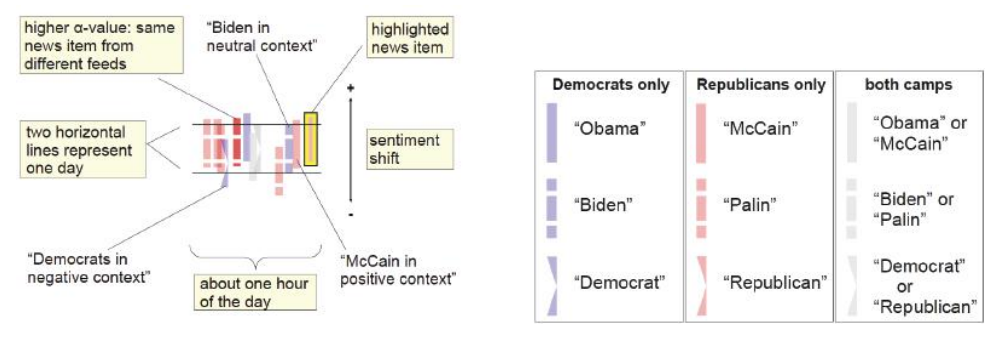
\includegraphics[width=0.9\textwidth]{17.png}
        \caption{Trực quan hóa phân tích cảm xúc \cite{440},
        Các mục tin tức được vẽ dọc theo trục thời gian.
        Hình dạng và màu sắc cho biết từng mục thuộc về danh mục nào và vị trí theo trục thẳng đứng phụ thuộc vào điểm số cảm xúc được xác định tự động của mục đó.
        Các đối tượng trực giác biểu diễn các mục tin tức được tô màu bán trong suốt để làm cho các mục chồng vào nhau dễ phân biệt hơn.}
        \label{fig:17}
    \end{figure}
\end{frame}

\subsection{Biểu diễn các mối quan hệ}

\begin{frame}{Biểu diễn các mối quan hệ}
	\begin{itemize}
		\item Jigsaw \cite{155} cũng bao gồm chế độ xem đồ thị thực thể (hình \ref{fig:18}) trong đó người dùng có thể điều hướng đồ thị của các thực thể và tài liệu có liên quan.
		\item Trong Jigsaw, các thực thể được kết nối với các tài liệu mà chúng xuất hiện.
		\item Chế độ xem đồ thị của Jigsaw không hiển thị toàn bộ tập tài liệu nhưng cho phép người dùng mở rộng dần dần đồ thị bằng cách chọn các tài liệu và thực thể mà họ quan tâm (hình \ref{fig:19})
	\end{itemize}
\end{frame}

\begin{frame}{Biểu diễn các mối quan hệ}
	\begin{figure}[h!]
        \centering
        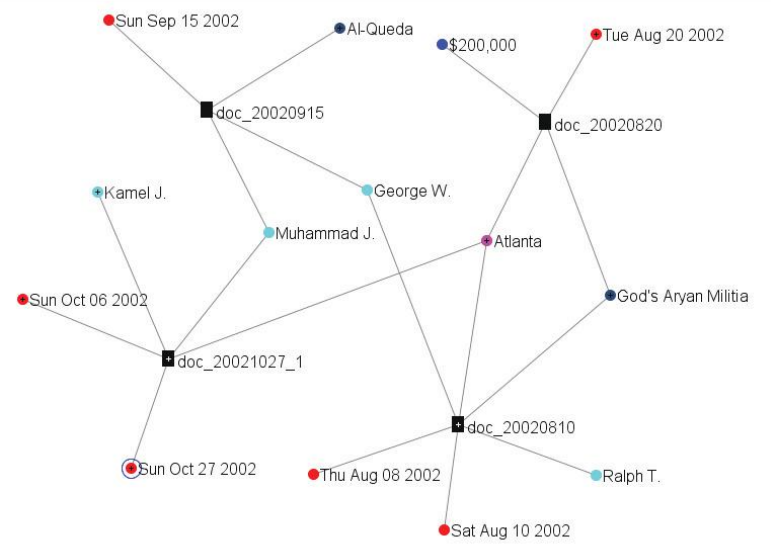
\includegraphics[width=0.65\textwidth]{18.png}
        \caption{Chế độ xem đồ thị Jigsaw, thể hiện các kết nối giữa các thực thể và tài liệu được đặt tên \cite{155}.}
        \label{fig:18}
    \end{figure}
\end{frame}

\begin{frame}{Biểu diễn các mối quan hệ}
	\begin{figure}[h!]
        \centering
        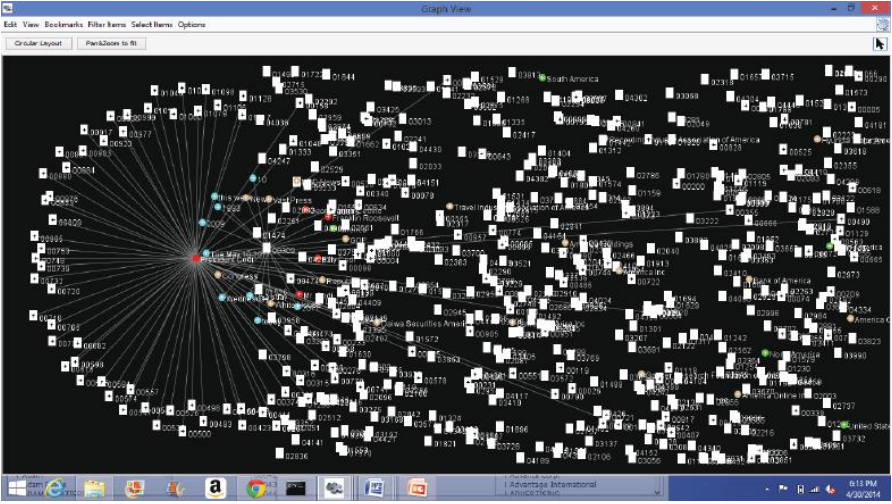
\includegraphics[width=0.8\textwidth]{19.png}
        \caption{Chế độ xem đồ thị phân cụm trong Jigsaw lọc các tài liệu có các thực thể cụ thể.
        Di chuột qua một thực thể xác định dữ liệu về tài liệu.
        Màu sắc đại diện cho giá trị tokens.}
        \label{fig:19}
    \end{figure}
\end{frame}

\begin{frame}{Biểu diễn các mối quan hệ}
	\begin{itemize}
		\item Chế độ xem danh sách trong Jigsaw là chế độ xem thay thế cho chế độ xem đồ thị ở chỗ cho phép người dùng khám phá những mối quan hệ giữa nhiều loại thực thể và tài liệu.
		\item Được minh họa trong hình \ref{fig:20}, khi người dùng chọn các mục mà họ quan tâm, chế độ xem danh sách vẽ các đường kết nối thể hiện mối quan hệ của chúng.
	\end{itemize}
\end{frame}

\begin{frame}{Biểu diễn các mối quan hệ}
	\begin{figure}[h!]
        \centering
        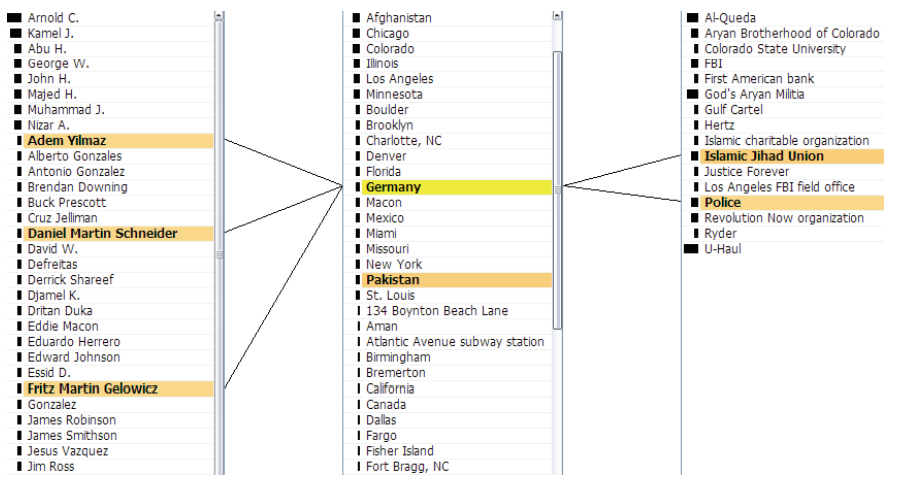
\includegraphics[width=0.9\textwidth]{20.png}
        \caption{Chế độ xem danh sách Jigsaw, hiển thị các kết nối giữa mọi người (bên trái), các địa điểm (giữa) và các tổ chức (bên phải) \cite{155}.}
        \label{fig:20}
    \end{figure}
\end{frame}

\section{Tài liệu tham khảo}
\begin{frame}[allowframebreaks]{Tài liệu tham khảo}
    \printbibliography
\end{frame}
\end{document}

